\sloppy
\chapter{SPECIFIKACIJA KORISNIČKIH ZAHTJEVA}

\sloppy
\section*{Kontrola verzija}


\noindent Arman Bašović - prikupljanje korisničkih zahtjeva, kreiranje ankete.

\noindent Tarik Hastor - kreiranje ankete.

\noindent Edin Živojević - poslovni procesi.

\sloppy
\section{Prikupljanje korisničkih zahtjeva}  
\subsection{Preliminarni funckionalni zahtjevi}
Na osnovu inicijalnog opisa projekta i analize konkurentskih sistema možemo zaključiti da su  \textbf{preliminarni funkcionalni zahtjevi} sljedeći:

\begin{itemize}
    \item \textbf{Online prodaja i rezervacija karata s višestrukim načinima plaćanja}: Omogućava korisnicima izbor predstava, pregled rasporeda, odabir sjedišta, te integrisani proces plaćanja uz podršku za kreditne kartice, \emph{Google Pay} i \emph{PayPal}. Uključuje primjenu popusta, korištenje lojalnih kartica i jednostavan tok od rezervacije do finalizacije transakcije.

    \item \textbf{Pregled predstava}:
    Omogućava korisnicima pregled predstojećih predstava, filtriranje prema žanru, datumu i popularnosti, te odabir predstave i sjedišta.

    Admin može dodavati, uređivati i brisati predstave, ažurirati raspored i dostupna sjedišta, te upravljati popustima i promocijama.

    \item \textbf{Korisnički profil}: Registracija, prijava, praćenje historije kupovina i personalizovanje profila.

    \item \textbf{Interaktivni forum}: Registrovani korisnici mogu ostavljati ocjene (1–5 zvjezdica) i komentare uz predstave, dok gosti imaju pristup samo čitanju. Komentari se automatski prikazuju uz predstavu, s mogućnošću dijeljenja na društvenim mrežama i \emph{real-time} ažuriranjem bez potrebe za osvježavanjem stranice.  

    \item \textbf{Integracija društvenih mreža}: Dijeljenje događaja na \emph{Instagram/TikTok} i prijava preko društevnih profila.

    \item \textbf{Marketing i obavještenja}: Slanje promotivnih obavijesti putem \emph{e-maila} i \emph{SMS-a}, te personalizovane ponude.
\end{itemize}

\subsection{Akteri sistema}
U kontekstu razvijanja informacionog sistema za Pozorište mladih, identifikovani su sljedeći ključni akteri:

\begin{itemize}
    \item \textbf{Gost (Neregistrovani korisnik)} 
    \begin{itemize}
        \item Opis: Korisnik koji pristupa sistemu bez registracije.
        \item Uloga: 
            \begin{itemize}
                \item Registracija
                \item Pregled repertoara i rasporeda predstava.
                \item Čitanje sadržaja foruma (ocjene, komentari, mediji).
                \item Ograničenja: 
                    \begin{itemize}
                        \item Nema mogućnosti rezervacije ili kupovine karata.
                        \item Nema prava na pisanje komentara ili sudjelovanje u forum diskusijama.
                    \end{itemize}
            \end{itemize}
    \end{itemize}
    
    \item \textbf{Registrovani korisnik}
    \begin{itemize}
        \item Opis: Korisnik sa kreiranim nalogom.
        \item Uloga: 
            \begin{itemize}
                \item Kupovina i rezervacija karata.
                \item Pisanje komentara i ocijenjivanje predstava na forumu.
                \item Korištenje lojalnog programa i personalizovanih preporuka.
            \end{itemize}
    \end{itemize}
    
    \item \textbf{Administrator}
    \begin{itemize}
        \item Opis: Zaposleni pozorišta zadužen za upravljanje sistemom.
        \item Uloga: 
            \begin{itemize}
                \item Ažuriranje repertoara i rasporeda.
                \item Moderacija foruma (uklanjanje neprimjerenih komentara).
                \item Upravljanje korisničkim nalozima i tehnička podrška.
            \end{itemize}
    \end{itemize}
\end{itemize}
\subsection{Analiza ankete}  
Anketa je sprovedena radi validacije preliminarnih funkcionalnosti i identifikacije dodatnih zahtjeva klijenata. Rezultati su potvrdili osnovne module projekta, ali su istaknuli i nove potrebe koje će biti uključene u dalji razvoj.  
U nastavku su detaljni odgovori i implikacije, s \textbf{dodacima na preliminarne funkcionalnosti} (1–2) i \textbf{novim funkcionalnostima} (3–6) identifikovanim kroz anketu.  

\begin{figure}[htbp]
  \centering 
  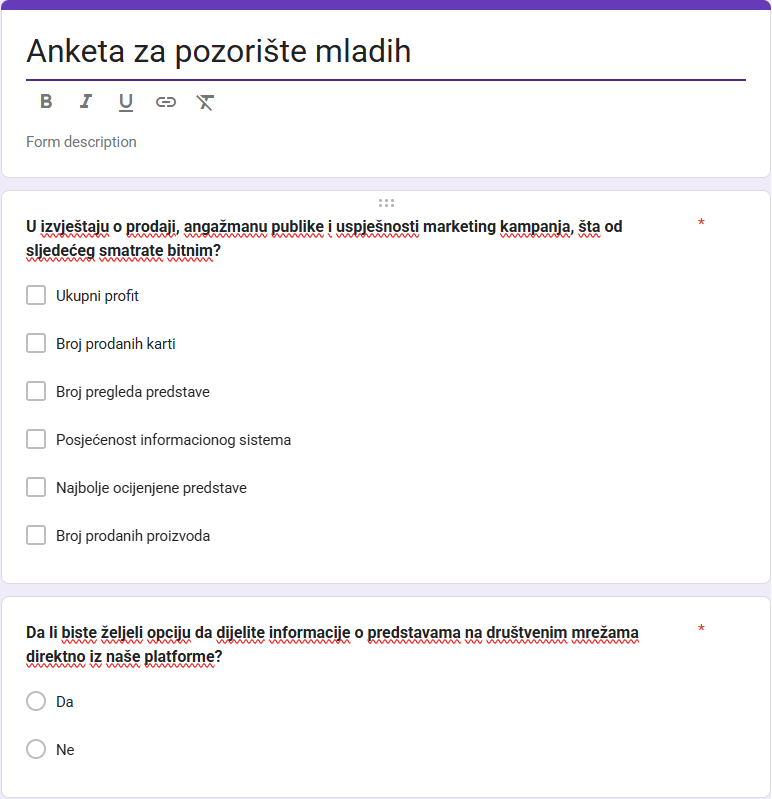
\includegraphics[width=0.8\textwidth]{Slike/Anketa.png} 
  \caption{Slika ankete} 
  \label{fig:anketa} 
\end{figure}

\subsubsection*{Dodaci na preliminarne funkcionalnosti}  

\paragraph*{1. Online prodaja i rezervacija karata}~\\
\textbf{Pitanje:}  
\emph{,,Da li biste voljeli odabir sjedišta preko interaktivne mape?''}  

\textbf{Odgovori klijenata:}  
\begin{itemize}  
    \item Da (100\% podrške).  
\end{itemize}  

\textbf{Implikacije:}  
\begin{itemize}  
    \item \textbf{Dodatak}: 2D/3D mapa sale s mogućnošću klika na sjedište i pregledom cijene.  
\end{itemize}  

\paragraph*{2. Integracija društvenih mreža}~\\
\textbf{Pitanje:}  
\emph{,,Da li biste željeli opciju da dijelite informacije o predstavama na društvenim mrežama direktno iz platforme?''}  

\textbf{Odgovori klijenata:}  
\begin{itemize}  
    \item Da (100\% podrške).  
\end{itemize}  

\textbf{Implikacije:}  
\begin{itemize}  
    \item \textbf{Dodatak}: Implementacija "dijeli" dugmadi za \emph{Facebook, Instagram} i \emph{TikTok}.  
\end{itemize}  

\subsubsection*{Nove funkcionalnosti (identifikovane anketom)}  

\paragraph*{3. Notifikacije o novim predstavama i ponudama}~\\  
\textbf{Pitanje 1:}  
\emph{,,Da li biste željeli mogućnost prilagodbe izgleda profila (npr. tema boja, notifikacije)?''}  

\textbf{Odgovori klijenata:}  
\begin{itemize}  
    \item 50\%: ,,Samo za notifikacije''  
    \item 50\%: ,,Da, želim personalizovati iskustvo''  
\end{itemize}  

\textbf{Pitanje 2:}  
\emph{,,Koliko su vam bitne automatske notifikacije korisnicima o predstavama?''}  

\textbf{Odgovori klijenata:}  
\begin{itemize}  
    \item 50\%: 4/5  
    \item 50\%: 5/5  
\end{itemize}  

\textbf{Implikacije:}  
\begin{itemize}  
    \item \textbf{Nova funkcionalnost}: Konfigurabilne notifikacije (\emph{e-mail/SMS/push}) s ograničenom personalizacijom.  
\end{itemize}  

\paragraph*{4. Višekanalna korisnička podrška i komunikacija}~\\  
\textbf{Pitanje:}  
\emph{,,Koje vidove komunikacije preferirate sa korisnicima?''}  

\textbf{Odgovori klijenata:}  
\begin{itemize}  
    \item \emph{Chatbot}  
    \item \emph{E-mail}  
\end{itemize}  

\textbf{Implikacije:}  
\begin{itemize}  
    \item \textbf{Nova funkcionalnost}: \emph{Chatbot} koji se nalazi u vidu ikonice na \emph{homepage-u}, korisnici mu mogu postavljati pitanja vezano za korištenje platforme sistema.  
\end{itemize}  

\paragraph*{5. Moderacija foruma}~\\  
\textbf{Pitanje:}  
\emph{,,Da li želite da se forum moderira od strane administratora?''}  

\textbf{Odgovori klijenata:}  
\begin{itemize}  
    \item Da (100\% podrške).  
\end{itemize}  

\textbf{Implikacije:}  
\begin{itemize}  
    \item \textbf{Nova funkcionalnost}: Alati za brisanje komentara, blokiranje korisnika i postavljanje forum pravila.  
\end{itemize}  

\paragraph*{6. Detaljna analitika i izvještavanje za administratore}~\\
\textbf{Pitanje:}  
\emph{,,Šta od sljedećeg smatrate bitnim u izvještaju o prodaji, angažmanu publike i uspješnosti marketing kampanja?''}  

\textbf{Odgovori klijenata:}  
\begin{itemize}  
    \item Ukupni profit  
    \item Broj prodanih karata  
    \item Najbolje ocijenjene predstave  
\end{itemize}  

\textbf{Implikacije:}  
\begin{itemize}  
    \item \textbf{Nova funkcionalnost}: Izvještaji s graficima i tabelama za ključne metrike.  
\end{itemize}  

\sloppy
\section{Poslovni procesi}

\sloppy
\subsection{PP1: Upravljanje repertoarom i prodajom karata}

Poslovni proces \textit{Upravljanje repertoarom i prodajom karata}, pokriva sve aspekte planiranja, prezentacije i prodaje predstava. Ovo uključuje kreiranje repertoara od strane administratora, definisanje rasporeda, realizaciju online prodaje i rezervacije karata. Na slici \ref{fig:pp1} je prikazan \textit{use-case} dijagram koji ilustruje poslovni proces. Obuhvaćene funkcionalnosti:

\begin{enumerate}
    \item Kreiranje i uređivanje korisničkih profila 
    \item Pregled i filtriranje trenutnih predstava 
    \item Online prodaja i rezervacija karata s višestrukim načinima plaćanja

\end{enumerate}

\begin{figure}[!htb]
    \centering
    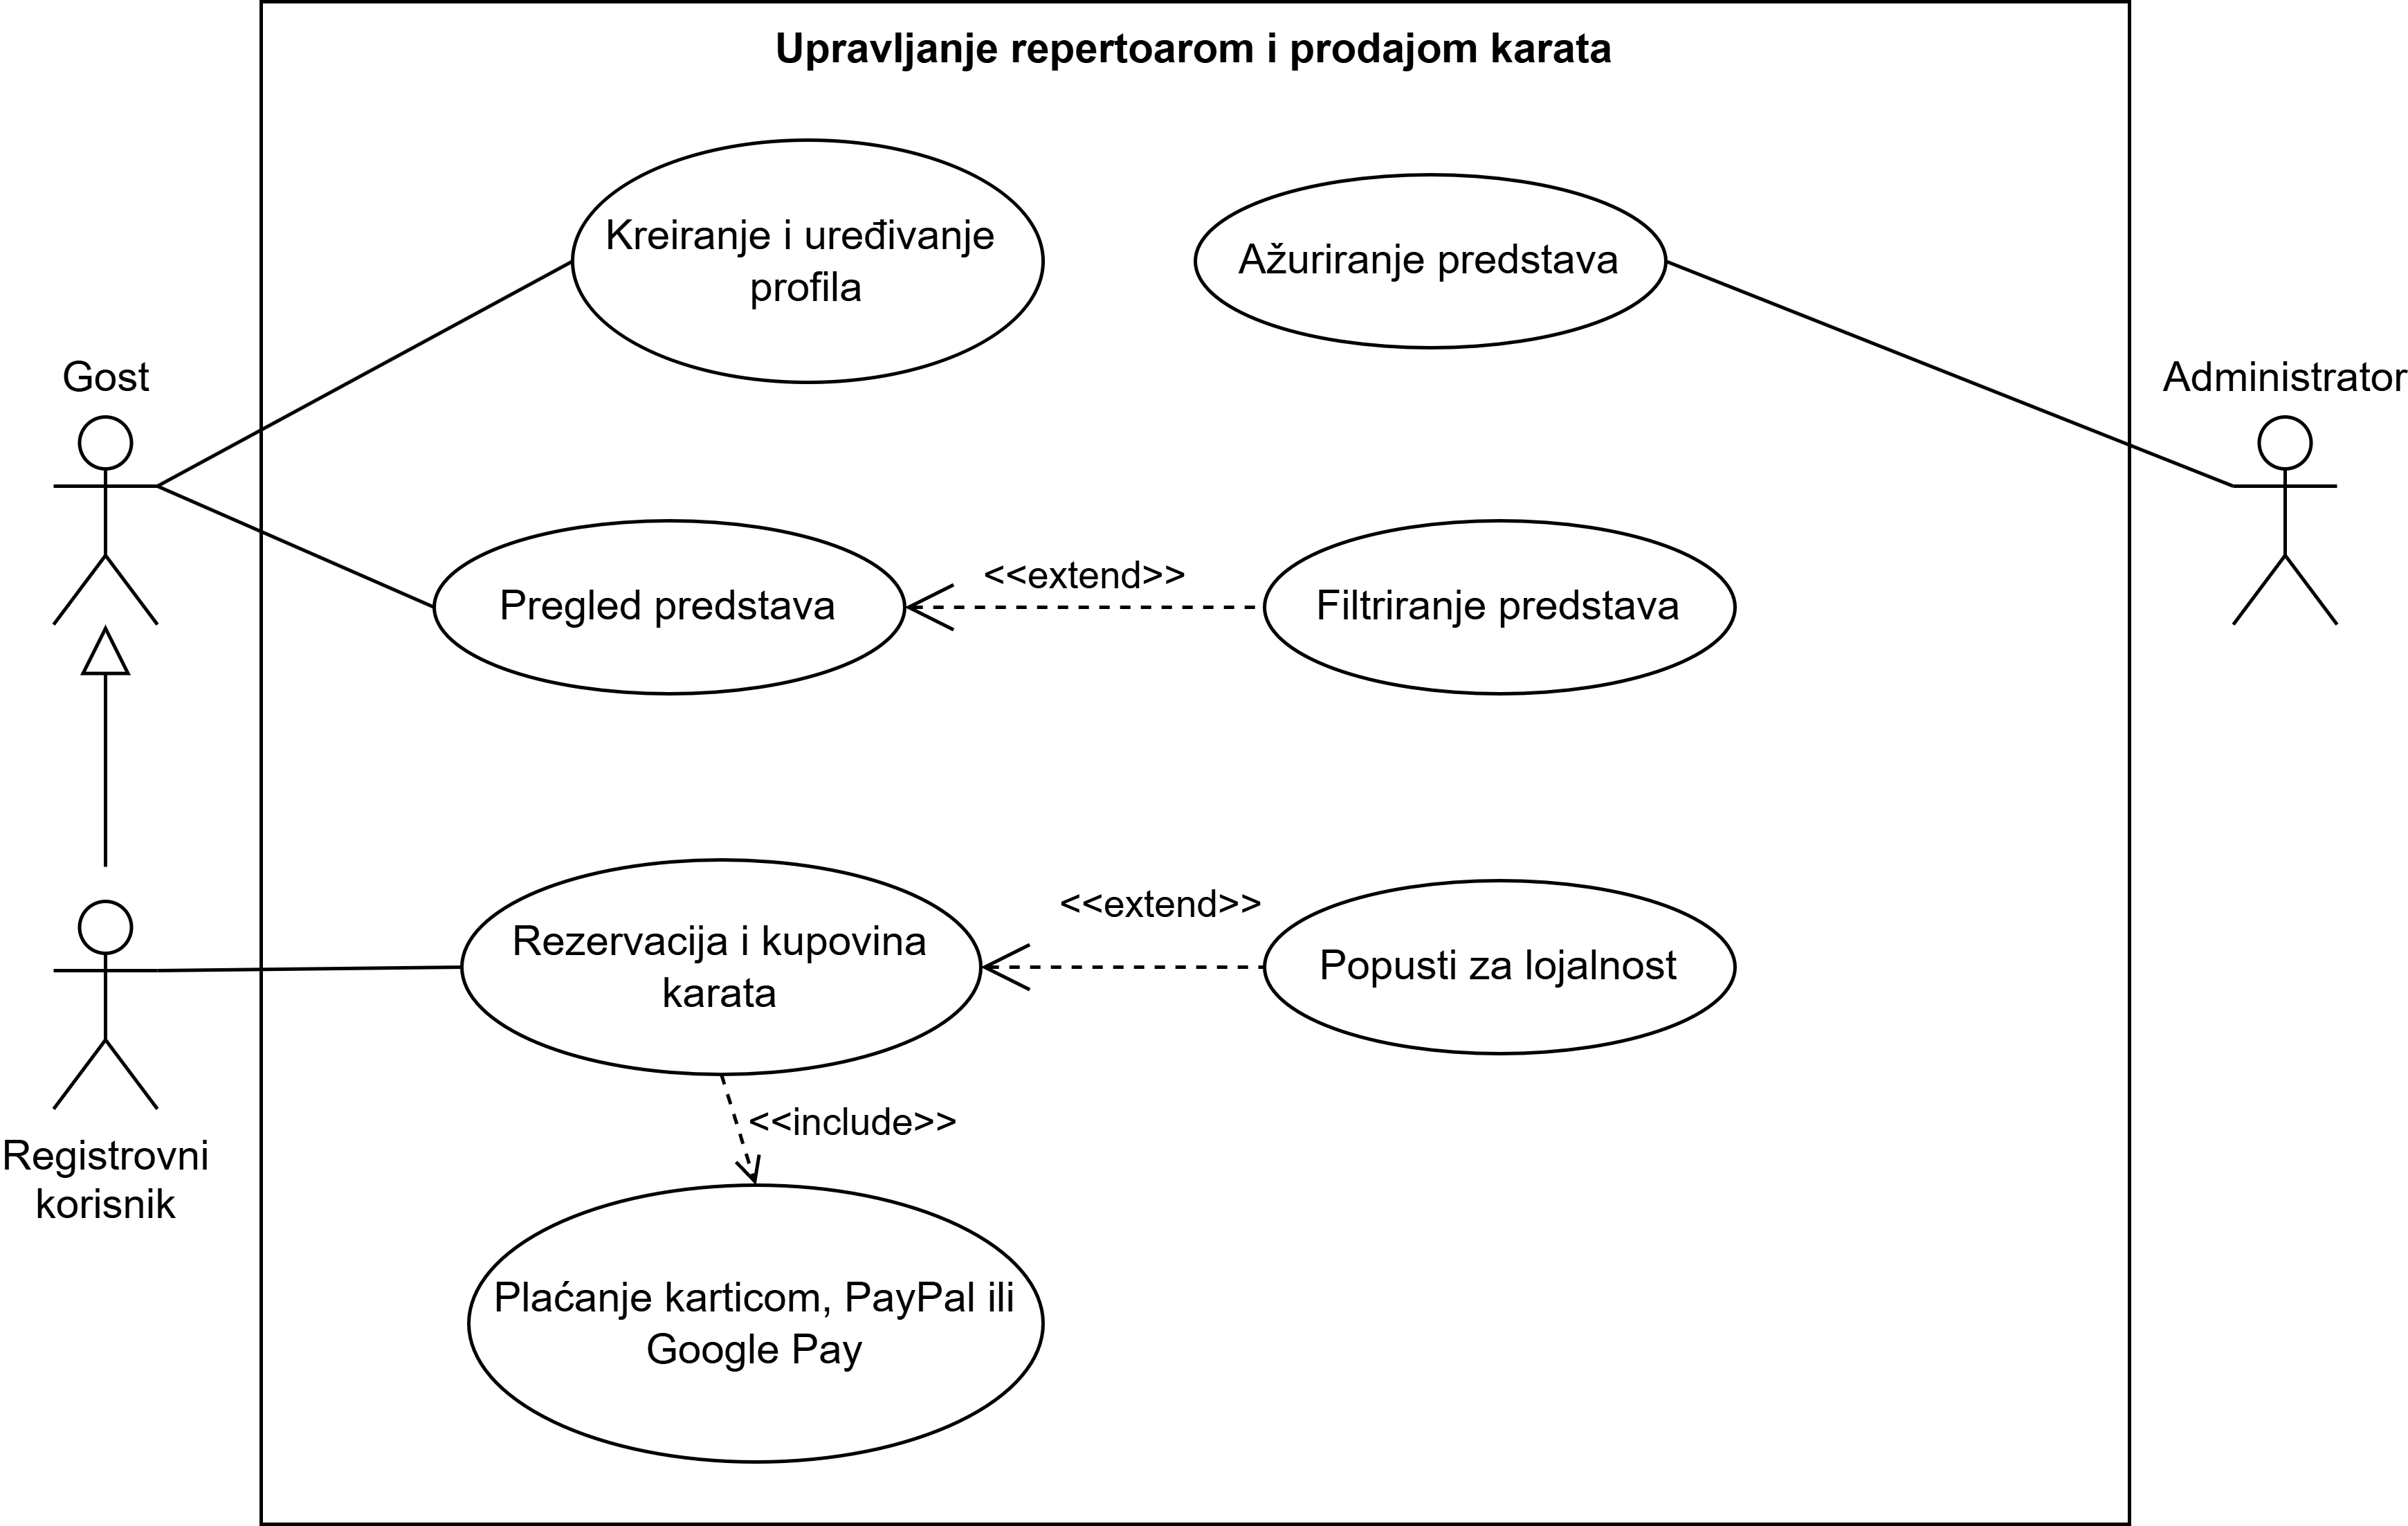
\includegraphics[width=1\linewidth]{Slike/Poslovni procesi/PP1.drawio.png}
    \caption{\textit{Use-case} dijagram za poslovni proces: \textit{Upravljanje repertoarom i prodajom karata}}
    \label{fig:pp1}
\end{figure}

\pagebreak
\subsection{PP2: Forum za predstave}

Proces \textit{Forum za predstave} pruža platformu za razmjenu mišljenja i dijeljenje utisaka sa predstava, tako što omogućava korisnicima da dodaju recenzije i komentare za pojedine predstave. Na slici \ref{fig:pp2} je prikazan \textit{use-case} dijagram koji ilustruje poslovni proces. Funkcionalnosti obuhvaćene ovim modulom:

\begin{enumerate}
    \item Pregled i dodavanje ocjena i komentara za predstave 
    \item Moderacija foruma od strane administratora
\end{enumerate}

\begin{figure}[!htb]
    \centering
    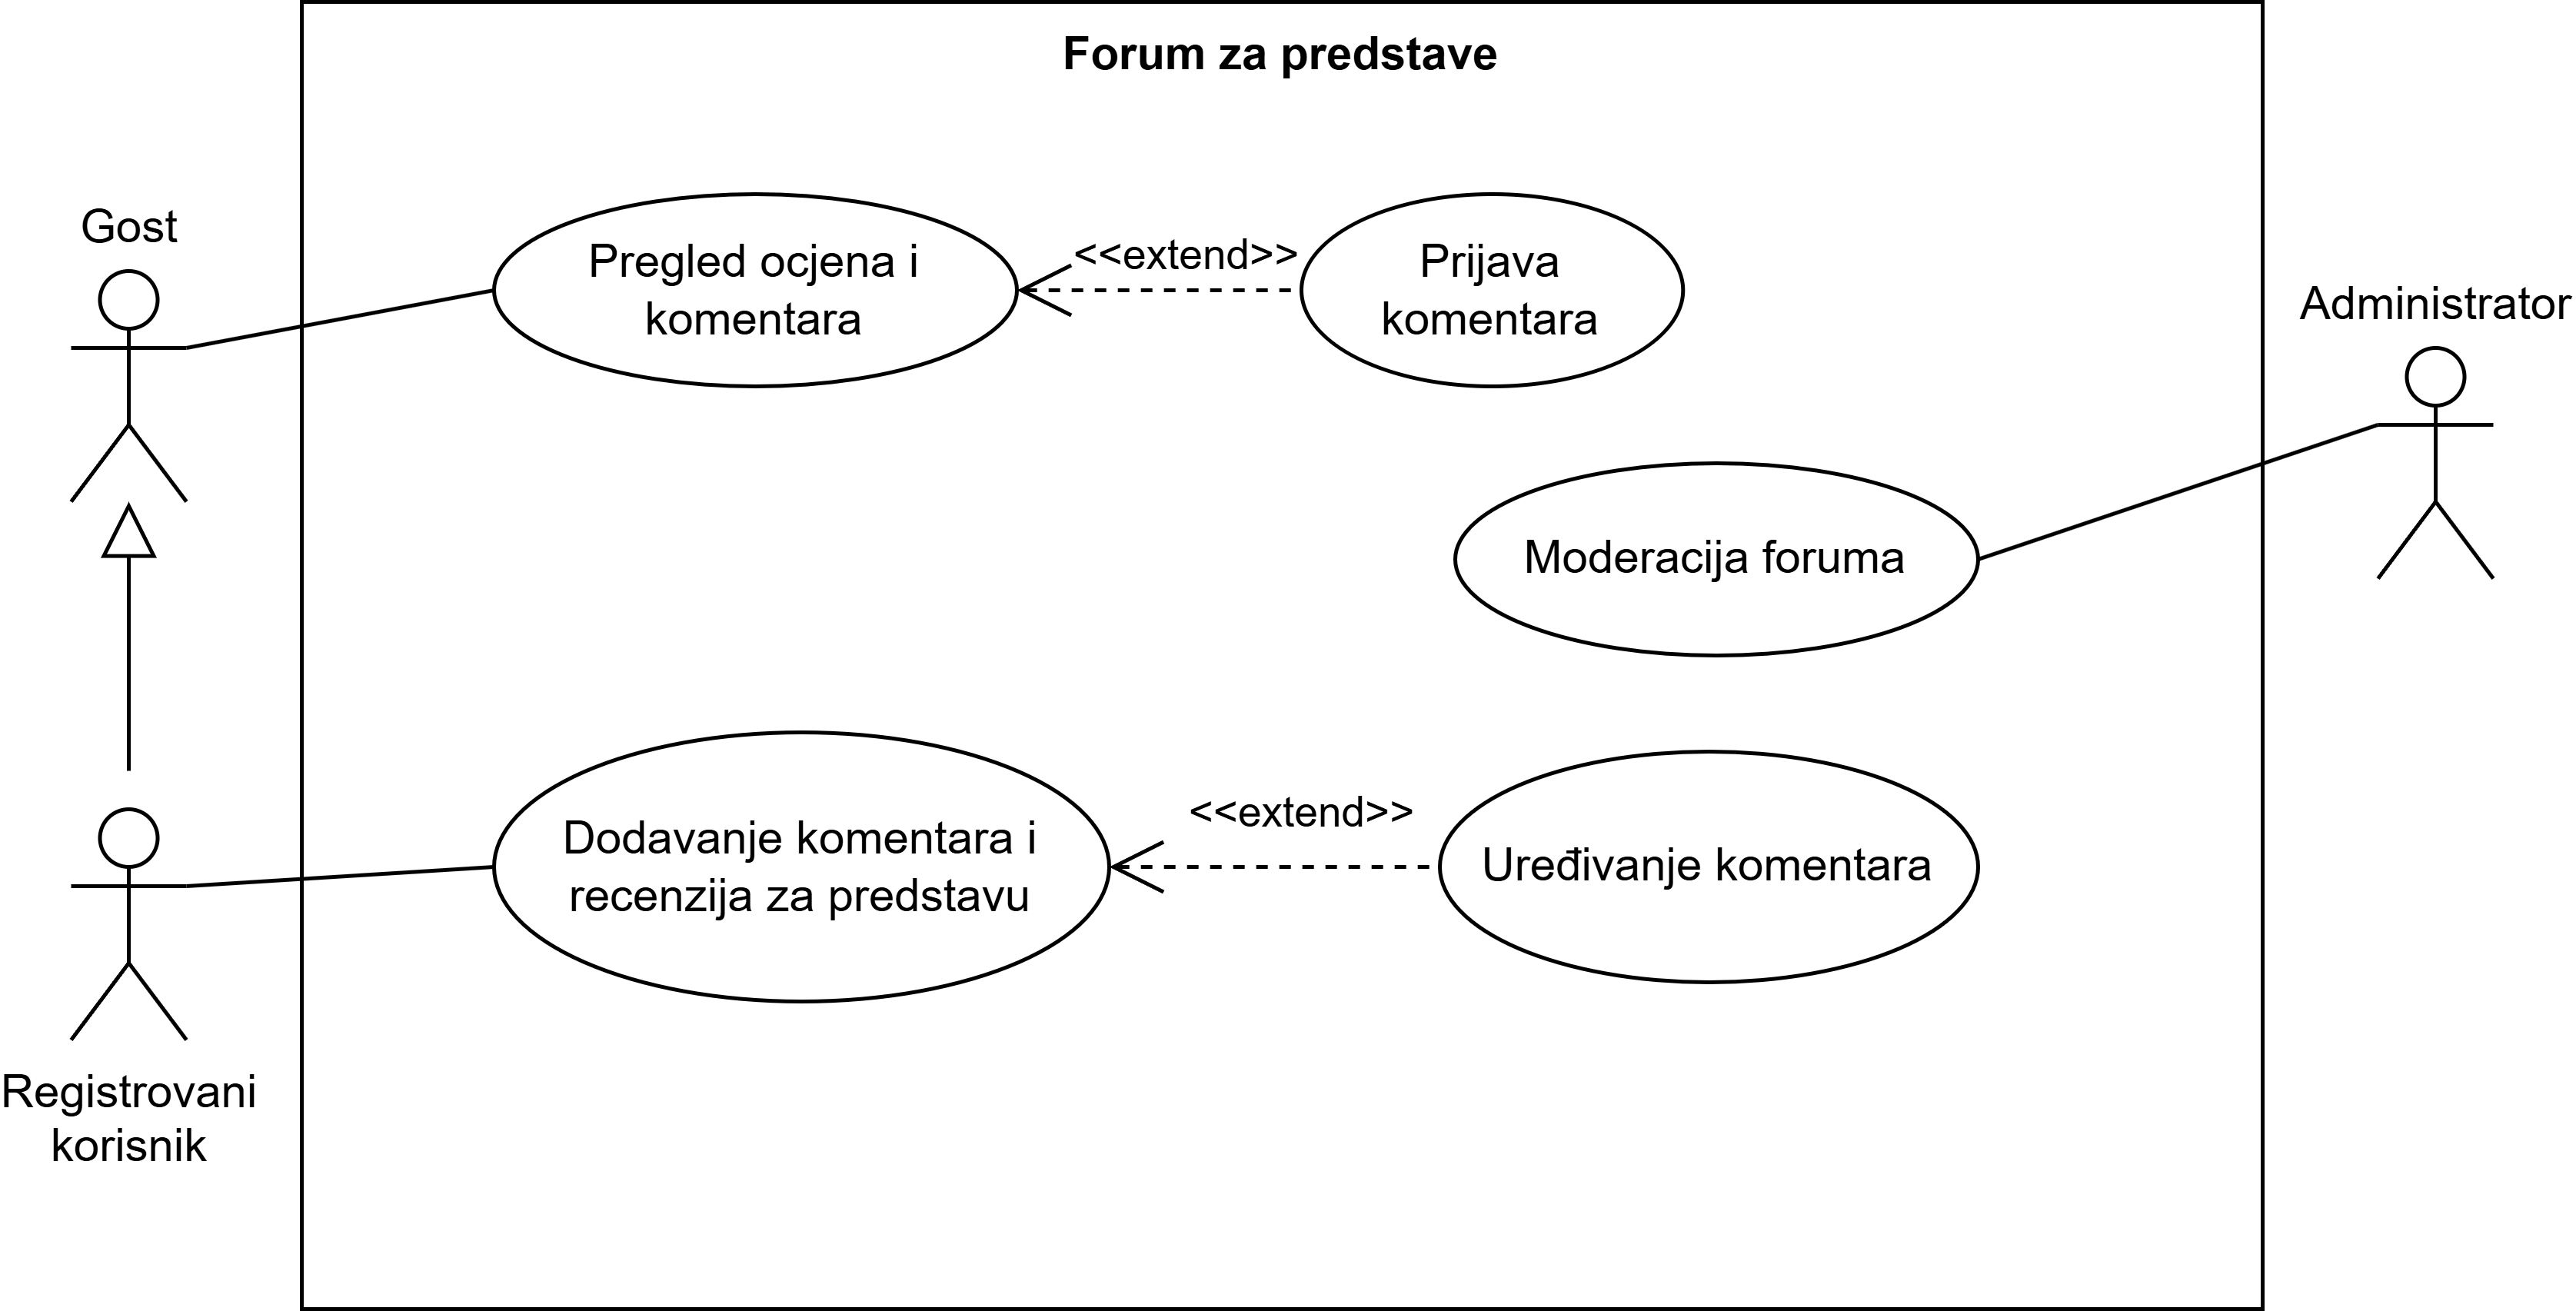
\includegraphics[width=0.8\linewidth]{Slike/Poslovni procesi/PP2.drawio.png}
    \caption{\textit{Use-case} dijagram za poslovni proces: \textit{Forum za predstave}}
    \label{fig:pp2}
\end{figure}

\subsection{PP3: Marketing i korisnička podrška}

Poslovni proces \textit{Digitalni marketing i komunikacija} integriše različite načine promocije, uključujući ciljane obavijesti i povezivanje sa društvenim mrežama, te omogućava prikupljanje povratnih informacija putem izvještaja. Također je omogućena korisnička podrška putem \textit{Chatbot}-a. Na slici \ref{fig:pp3} je prikazan \textit{use-case} dijagram koji ilustruje poslovni proces. Obuhvaćene funkcionalnosti:

\begin{enumerate}
    \item Dijeljenje sadržaja putem društvenih mreža
    \item Notifikacije o novim predstavama i ponudama
    \item Korisnička podrška putem \textit{Chatbot}-a
    \item Detaljna analitika i izvještavanje za administratore
\end{enumerate}

\newpage
\vspace*{0pt}
\begin{figure}[t!]
    \centering
    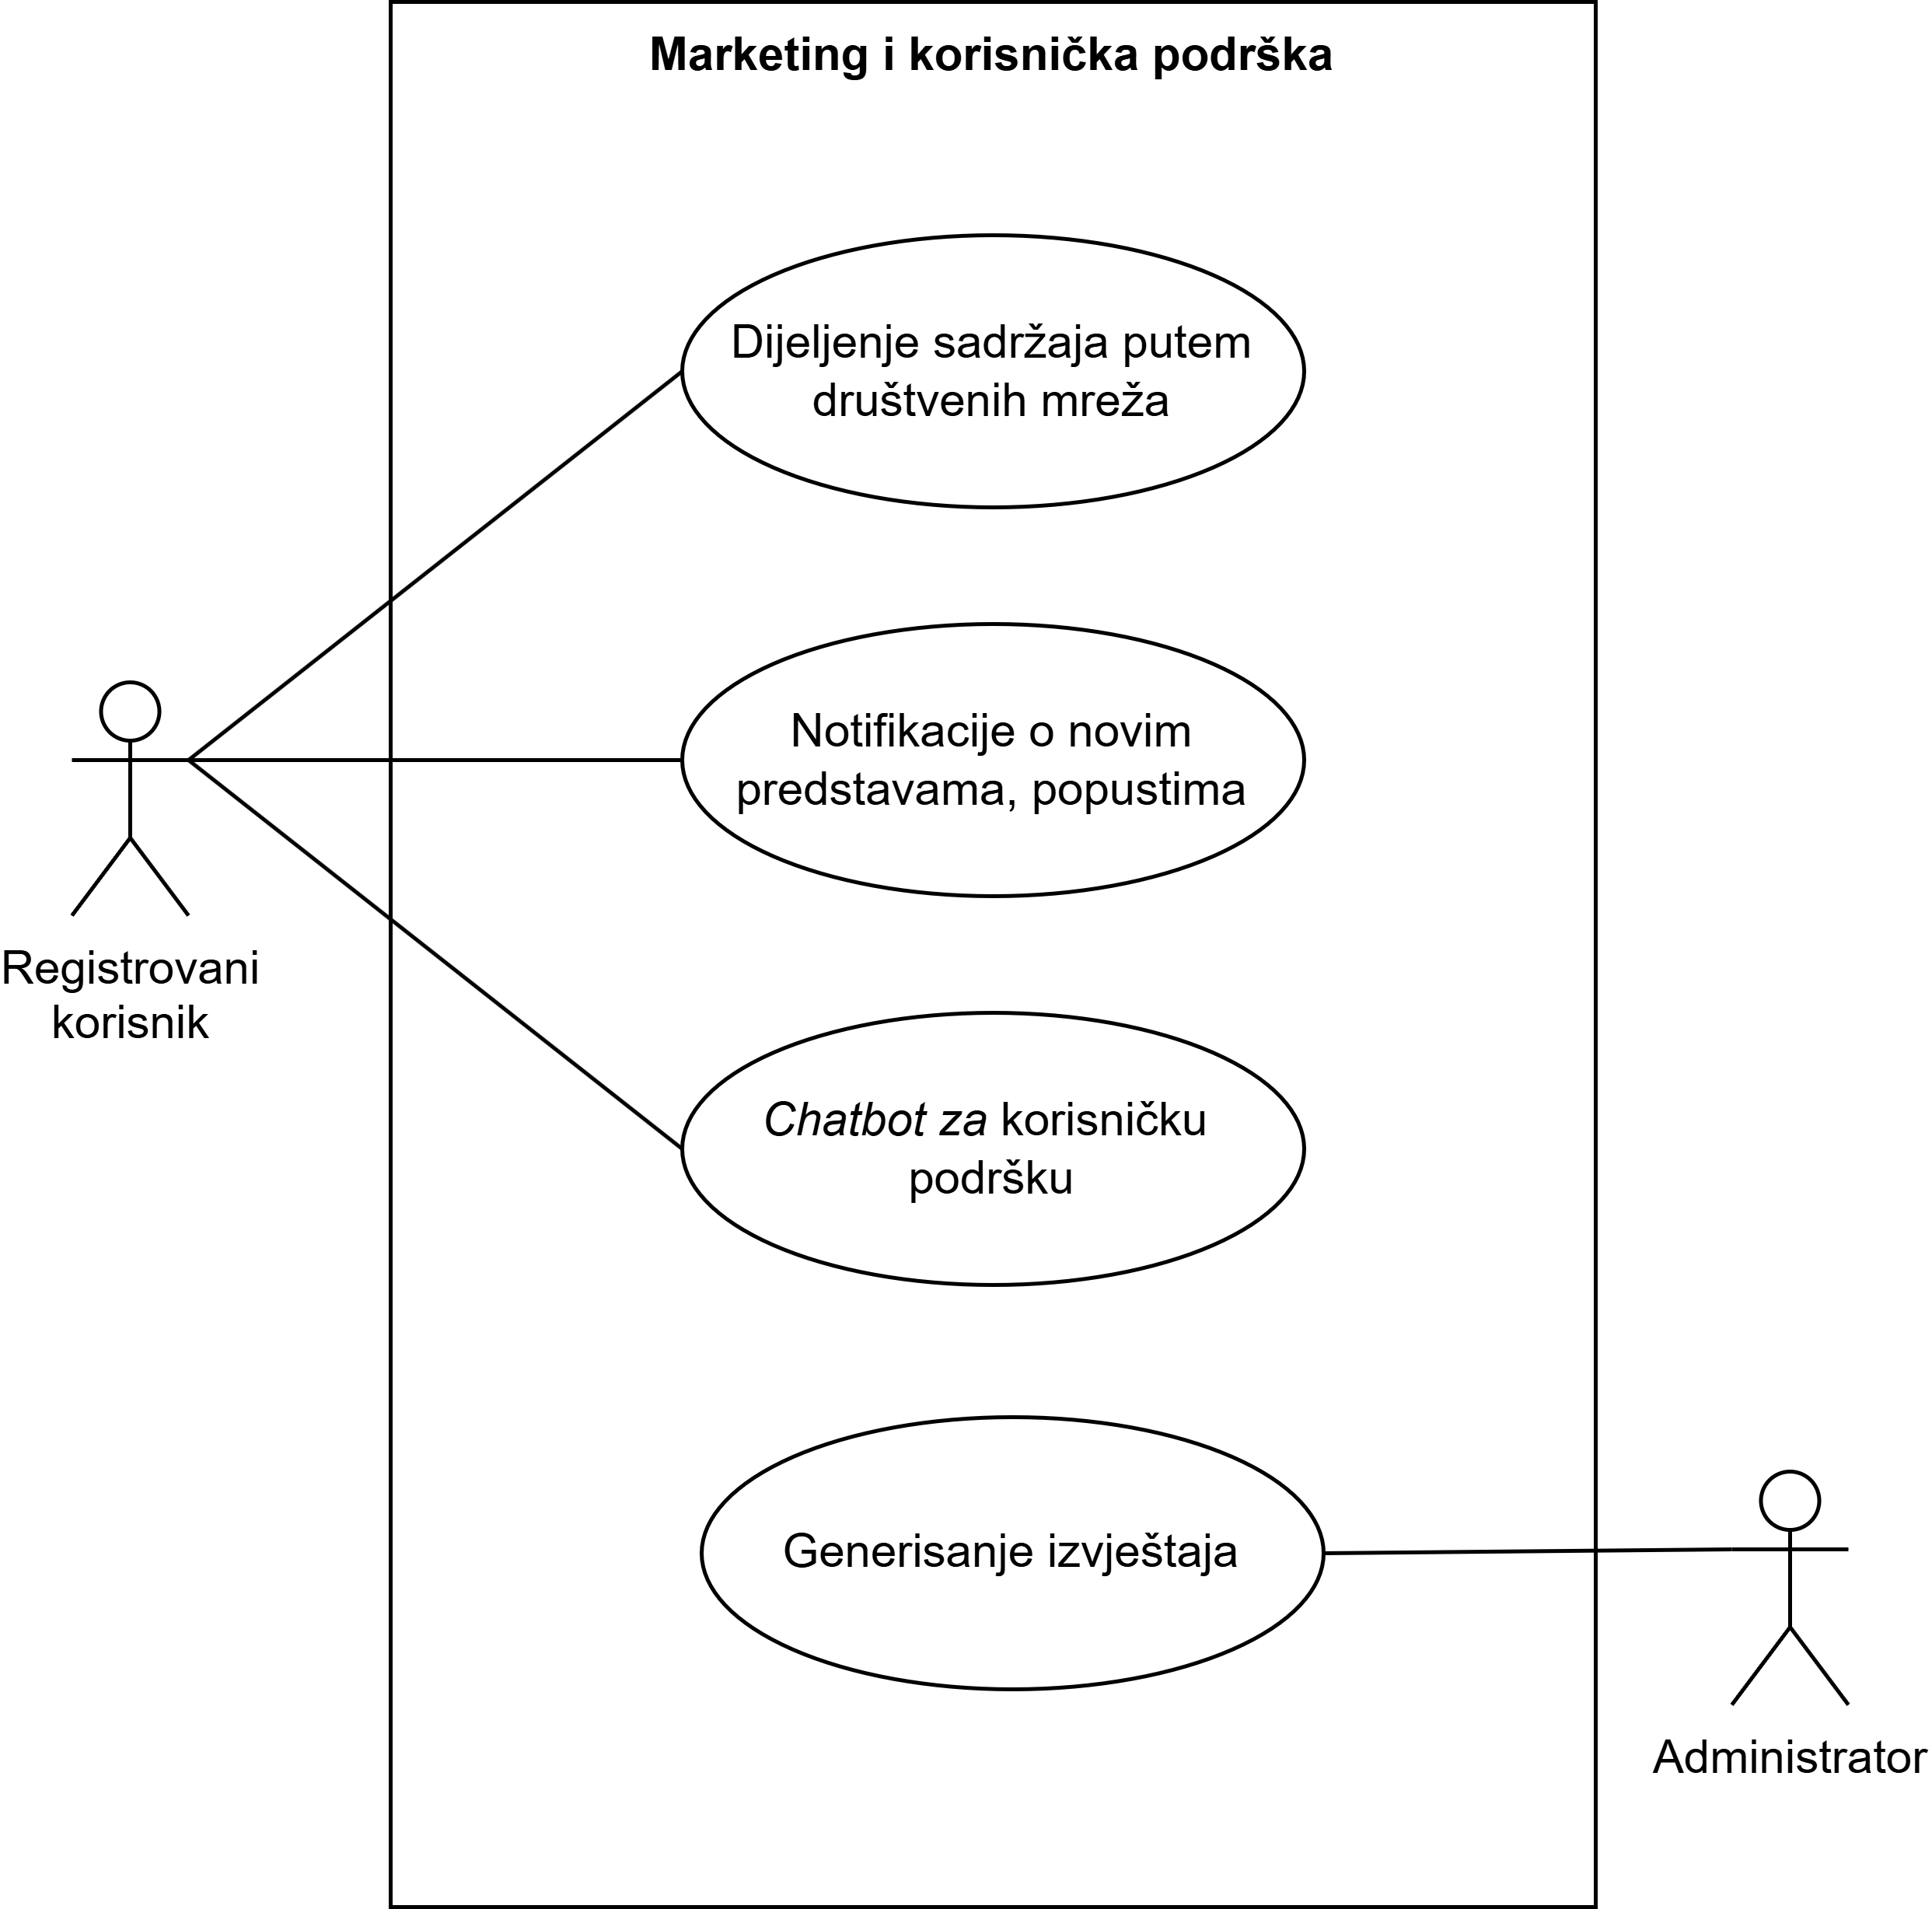
\includegraphics[width=0.6\linewidth]{Slike/Poslovni procesi/PP3.drawio.png}
    \caption{\textit{Use-case} dijagram za poslovni proces: \textit{Marketing i korisnička podrška}}
    \label{fig:pp3}
\end{figure}
\newpage